%Contributer: Kendal Sandridge
{\parindent0pt
\section{Spectral Clustering}

As of late Spectral Clustering has become exceedingly popular due to the quality of its clusters compared to other clustering algorithms.   It is possible to turn clustering into a graph problem, then solve it by figuring out the cut that splits our graph into the groups with high intracluster weights. One of the benefits of this formulation is that the data can be in any space, not just euclidean, and we can still perform clustering. \\

We can formulate the problem of spectral clustering with well defined inputs and outputs 
\textbf{Input:} 
- $x_1,...,x_n$ data points\\
- $w_{ij}$ similarity between points $x_i, x_j$ \\

\textbf{Goal}\\
- MINIMIZE intercluster weights\\
- MAXIMIZE intracluster weights\\



We first introduce the notion of a similarity graph. We can construct a similarity graph from a set of points $S$, and a similarity function that returns a value $s_{ij}$, the similarity from points $i, j \in S$. In this way we construct a graph $G = (V,E)$ where $V = S$ and $(i,j) \in E$ if $s_{ij} > 0$.  The weights of each edge in the weights matrix would be $s_{ij}$ if $s_{ij}$ is positive and 0 otherwise. There are actually many ways of constructing the weight matrix $W$ of $G$. A few are listed below:\\

\textbf{Methods of creating W}
\begin{itemize}
	\item k-NN graph
	\item $\epsilon$-neighbor graph
	\item Gaussian kernel $w_{ij} = exp(\dfrac{-\lVert x_i - x_j\rVert ^2}{2 \sigma ^2})$
\end{itemize}

A few facts about the weights matrix is that if $w{ij} = 1 \Longleftrightarrow (i,j) \in E$, then $W$ is the usual adjacency matrix. Also $W$ is symmetric. \\


We can define the degree of the a vertex, $v \in V$ to be:
\begin{center}
	\[ d_i := \sum_{j \in V} w_{ij}\]
\end{center}

From this we can also define a degree matrix, $D$:
\begin{center}
	$D = diag(d_i, ..., d_n)$	
\end{center}

\textbf{Useful Notation}\\
It is also helpful to define an edge function $E(S,T)$:
\begin{center}
	Given that $S, T \subset V$ $ E(S,T) := \{(i,j) \in E : i \in S, j \in T\}$\\
\end{center}

We denote the compliment of a set of vertices, $\bar{S}$ as:
\begin{center}
	$\bar{S} := S \setminus V$
\end{center}

For shorthand we denote:
\begin{center}
	$\delta S = E(S, \bar{S})$
\end{center}

It is also important to have a notion of size for a set of vertices. The first is simply the cardinality of the set. The second is the volume of the set defined below.
\textbf{Measures of Size} $S \subset V$: \\
\begin{center}
	\item \[vol(S) := \sum_{i \in S} d_i = \sum_{\substack{i\in S \\
			j\in V}} w_{ij} = weight(E(S, V))\]
\end{center}


\textbf{The MINCUT Problem}\\
\[  \underset{{\emptyset \varsubsetneq S \varsubsetneq V}}{\mathrm{min}}  weight(E(S,\bar{S})) = weight(\delta S) \]\\

\textbf{Fact} \textit{(Stoer-Wagner, 1995)}. There is an efficient algorithm that solves MINCUT.\\
	
	Question: Is this good for clustering?\\
	A: No. We can try to "balance" the size of each partition but turns out the problem become NP-hard \textit{(Wagner \& Wagner 19)}\\
	
	\subsection{Spectral Graph Theory}
	At its heart, the graph Laplacian, L.
	
	\textbf{Review of Laplacian}
	$G = (V,E)$
	Dictionary between discrete calculus \& vector calculus:

	\begin{multicols}{2}
		\textbf{Discrete Calculus}\\
		\begin{itemize}
		\item $V$ is sparse  
		\item $\mathbb R^V$ is space of vertex functions\\
			 inner product space: $\langle f,g\rangle_v := \sum_{i\in V} f(i)g(i)$
		
		\item $\mathbb R^E$ is space of alternating vertex functions
			 \[X([i,j] = -X([j,i]) \textrm{for} (i,j) \in E \]
			inner product space: \[\langle X,Y\rangle_E := \sum_{e \in E} w_e X(e) Y(e) \]
		\item $d$ the derivative operator
		\[d: \mathbb R^V \rightarrow \mathbb R^E\]
		\[ df([i,j]) = f(j)-f(i)\]
		\item Dirichlet energy, measure of smoothness
		\[\mathcal E(f) := \langle df,df\rangle_E = \sum_{\substack{(i,j)\\
				{i < j}}} w_{ij} (f(i)-f(j))^2\]\\
		\end{itemize}
		\columnbreak
		\textbf{Vector Calculus}
		\begin{itemize}
			\item $\mathcal M$ is sparse
			\item $\mathcal C^{\infty}(\mathcal M; \mathbb R)$ space of functions 
			\item $\nabla$ gradient operator
			\item $\mathcal E(f) := \int_{\mathcal M} \lVert \nabla f \rVert ^2$
		\end{itemize}
	\end{multicols}
	Recall the adjoint.\\
	\begin{center}
		if $T: A \rightarrow B$ map of finite-dimension inner product spaces, then\\
		$\exists! T*: B \rightarrow A$ s.t. $\forall a \in A, b \in B, <a, Ta>_B = \langle T*b, a\rangle_A$
	\end{center}
	
	The Laplacian $L$ defined so that:
	\begin{center}
		$\langle df, df\rangle_E = \langle f,Lf\rangle_V$
	\end{center}
	
	Why consider L? In order to form an optimization problem!
	e.g. 
	\begin{center}
		$min \langle df, df\rangle_E $ \indent Lagrange Multipliers $\rightarrow Lf = \lambda f$\\
		s.t. \[ \lVert f \rVert ^2 = 1 \]
	\end{center}
	
	\textbf{Properties of Laplacian}
	\begin{enumerate}
		\item $L = D - W$
		\item $\mathbbm{1} \in ker(L)$
		\item $L \in Sym(\mathbbm R^{n\times n})$
		\item let $A \subset V$. $\mathbbm 1_A^T L \mathbbm 1_A = \sum_{(i,j) \in E} w_{ij} (\mathbbm  1_A(i - \mathbbm 1_A(j)) )^2 = weight(E(A, \bar{A})) $
	\end{enumerate}
	
	\subsection{Review of Spectral Theory: Geometric \& Variational Characterization of Eigenvalues}
	
	\begin{definition}
		Let $M \in \mathbb R^{n \times n}$. An eigenvector $v \in \mathbb R^n$ satisfies $v \neq 0, \exists\lambda \in \mathbb R $ s.t. $Mv = \lambda v$
		The eigenvalues of this matrix form its spectrum.
	\end{definition}
	
	\begin{theorem}[Spectral Theorem for Symmetric Matrices]
		
		Geometric characterization
		
		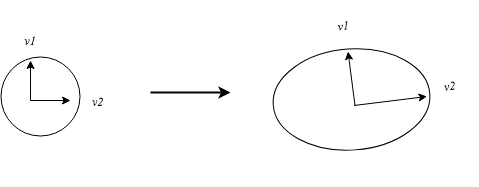
\includegraphics[width=0.8\textwidth]{chapter_3/files/spec_clust_diag.png}
	\end{theorem}
	
	\begin{definition}
		Let $v \neq 0 $ in $\mathbb R^n, \mathcal M \in Sym(\mathbb R{n \times n})$
		Rayleigh Quotient
		$\mathcal R(v) = \dfrac{v^T M v}{v^Tv}$
		
		Notice: $\mathcal R(\alpha v) = Rank(v) \forall \alpha \in \mathbb R \ \{0\}$, can assume $v \in S^{n-1}$
	\end{definition}
	
	
	\begin{theorem}[Variational Characterization]
		Let $M \in Sym(\mathbb R^{n\times n})$\\
		$\lambda_1 \leq ... \leq \lambda_n$ eigenvalues of M\\
		$\lambda_1 = min_{v \in S^{n-1}} Rank (v)$ let $v_1 = argmin$\\
		$\vdots$\\
		$\lambda_i = min_{\substack{ v \in S^{n-1}\\
				v \perp < v_1 ... v_{i-1} >}} $
	\end{theorem}
	Pf.
	
	\begin{exercise}
		let $M \in Sym(\mathcal R^{n \times n})$
		$min_{x} \sum_{i=1}^{n} x_i^T M x_i$ $min_(X) Tr(X^T M X)$ s.t. $X^TX = Id_{k\times k}$ 
		
		Q if $X$ minimizes this prob, is $X$ unique?\\
		A No. Let $U$ be an orthogonal matrix.  Consider $XU$. \\
		Claim: $XU$ is also optimal\\
		
		Fact $Tr(ABC) = Tr(BCA)$ \\
		
		\begin{center}
			$Tr(XU)^T M (XU)$\\
			$ Tr(X^T M X)$ given $(XU)^T(XU) = Id$
			$=Tr(X^TMX)$
		\end{center}
		
	\end{exercise}
}

